\section{Verwaltung von Test-Daten und Test-Systemen}\label{chap:testdataadministration}

%%%%%%%%%%%%%%%%
%
%    Verwaltung von Test-Daten und Test-Systemen
%
%%%%%%%%%%%%%%%%

An das Backend der Web-IDE ist eine eigene SAP HANA-Instanz angebunden.
Darin werden die Testdaten-Sets und Zugangsdaten für Test-Systeme hinterlegt.
Im folgenden geht es um das zugrundeliegende Schema, die Integration verschiedener Test-Systeme und das Pflegen der Test-Daten, insbesondere in Hinblick auf deren Gültigkeit.

\subsection{Datenschema für Testdaten-Sets}
Die Herausforderung beim Speichern der Testdaten-Sets liegt in der Wiederzuordnung zu den Variablen in der vom Entwickler geöffneten Quelltext-Datei.
Der in der Web-IDE genutzte Quelltext-Parser \cite{Horschig2014} nutzt symbolische Ausführung \cite{DBLP:journals/cacm/King76} zur Bestimmung von Variablen und deren eventuell bereits festgelegten Werten.
Die auf diesem Wege gefundenen Variablen bekommen eine eindeutige Kennzeichnung, die zum Identifizieren genutzt werden kann.
Sollten sie im Laufe des Programmflusses in mindestens ein SQL-Statement einfließen, werden sie als Test-Variablen betrachtet.
Eine Menge von Test-Variablen bildet zusammen mit dem Dateipfad und einem vom Entwickler angegebenen Namen ein Test-Set.
Diese Test-Sets können wiederum in Beziehung mit dem Test-System gebracht werden, auf dem die Performance-Analysen erfolgten, um die Abhängigkeit der System-Auswahl auf die Laufzeiten der Test-Sets zu berücksichtigen.
In Abbildung \ref{fig:erm} ist das dazugehörige Datenschema dargestellt.

\newcommand {\key}[1]{\underline{#1}}

\begin{figure}[ht]
	\centering
	\begin{tikzpicture}[node distance = 7em]
		\node [entity] (testset) {Test Set};
		\node [attribute] (tsid) [left of=testset] {\key{ID}} edge (testset);
		\node [attribute] (tsname) [above right of=testset] {Name} edge (testset);
		\node [attribute] (tsfilepath) [above left of=testset] {File Path} edge (testset);
		\node [relationship] (tshastv) [right of=testset] {has} edge (testset);
		\node [entity] (testvalue) [right of=tshastv] {Test Variable} edge [total] (tshastv);
		\node [attribute] (tvid) [above left of=testvalue] {\key{ID}} edge (testvalue);
		\node [attribute] (tvvariable) [above right of=testvalue] {Variable} edge (testvalue);
		\node [attribute] (tvvalue) [right of=testvalue] {Value} edge (testvalue);
		\node [relationship] (tshastsys) [below = 0.5cm of testset] {has} edge (testset);
		\node [entity] (testsystem) [below = 0.5cm of tshastsys] {Test System} edge [total] (tshastsys);
		\node [attribute] (tsysname) [left of=testsystem] {\key{Name}} edge (testsystem);
		\node [attribute] (tsyshost) [below right of=testsystem] {Host} edge (testsystem);
		\node [attribute] (tsysport) [below of=testsystem] {Port} edge (testsystem);
		\node [attribute] (tsysuser) [below left of=testsystem] {User} edge (testsystem);
		\node [attribute] (tsyspassword) [right = 0.5cm of testsystem] {Password} edge (testsystem);
	\end{tikzpicture}
	\caption{ER-Diagram für die Administration von Test-Sets und -Systemen}
	\label{fig:erm}
\end{figure}

\subsection{Caching und Gültigkeit von Test-Daten}
Um nicht für jede Vorschlaganfrage einen Datenbankzugriff durchzuführen, werden die Testdaten und Testdaten-Sets sowohl im Frontend als auch im Backend gecached.
Die Caches unterscheiden sich in der Hinsicht, dass es einen Frontend-Cache für jede Sitzung eines Entwicklers gibt, wohingegen der Backend-Cache global agiert.
Eine Anfrage für Testdaten-Vorschläge zu einer Spalte einer Relation wird dabei erst versucht durch den Frontend-Cache zu beantworten.
Sollten dort keine passenden Daten vorliegen, wird eine Anfrage an das Backend ausgelöst.
Dort versucht der Backend-Cache als erste Instanz diese Anfrage zu beantworten.
Sollten auch dort keine Daten vorliegen, werden die Vorschläge mithilfe der in Kapitel \ref{chap:testdatasuggestions} vorgestellten Algorithmen bestimmt und in den Caches hinterlegt.

Eine Herausforderung stellt das Überprüfen der Gültigkeit der Vorschläge und Testdaten-Sets dar.
Diese kann durch zwei Fälle beeinflusst werden: die Daten in der genutzten Datenbank werden verändert (erweitert, aktualisiert oder gelöscht) oder der Quelltext der Anwendung wird in einer Weise abgeändert, die die Variablen aus den SQL-Statements beeinflusst.

Für Ersteres gibt es Ansätze \cite{DBLP:conf/dasfaa/HarangsriSN97}, die kontinuierlich verändernde SQL-Statements nachverfolgen und dementsprechend ihren Algorithmus durch manuelles Hoch- bzw. Runterzählen der Anzahl von Einträgen in der betrachteten Relation anpassen.
Ein solches Vorgehen ist für die in Kapitel \ref{chap:testdatasuggestions} beschrieben Algorithmen nicht umsetzbar, da sie fest gekoppelt sind an die Werte in der Datenbank und nicht nur an ihre Anzahl.
Nichtsdestotrotz floss die Idee der Betrachtung von manipulierenden SQL-Statements mit in die Implementierung ein, indem ein Schwellwert für Datenveränderungen festgelegt wird (derzeit 10), ab dem eine Neubestimmung von Vorschlägen und initial berechneten Testdaten-Sets erfolgt.

Die Invalidierung der Daten durch Veränderung des dazugehörigen Quelltextes wurde im Zuge dieser Arbeit nicht betrachtet, ist aber als Weiterentwicklung geplant.
Die Schwierigkeit liegt darin, eine Granularität zu finden, auf der Änderungen zur Invalidierung führen, und gegebenenfalls diese Veränderung nachzuvollziehen.
Legt man die Granularitätsstufe auf das gesamte Dokument fest, würde dies dazu führen, dass die Test-Daten zu häufig als ungültig gekennzeichnet werden, obwohl das nicht zwangsläufig zutreffen muss.
Wählt man eine feine Granularitätsstufe (zum Beispiel alle Änderungen, die nur Variablen betreffen, die in SQL-Statements einfließen), so ist eine komplexe Nachverfolgung der Änderungen am Dokument über dessen verschiedene Revisionen notwendig.
Sollte ein Versionsverwaltungssystem für die Quelltext-Dateien genutzt werden, können dessen Informationen in der Nachverfolgung berücksichtigt werden.

\subsection{Integration mehrerer Test-Systeme}
Typischerweise dient nicht nur ein System als Grundlage für Performance-Analysen einer Geschäftsanwendung, sondern ein Auswahl an Systemen mit unterschiedlichen Ausstattungsmerkmalen.
Dies kann mehrere Gründe haben.
In Hinblick auf die Daten können so Datenschutz-Bestimmungen eingehalten oder auch Datensätze mit verschiedene Charakteristiken getestet werden.
Zum anderen kann so auch die Auswirkung verschiedener System-Konfigurationen auf die Performance der Anwendung geprüft werden, wodurch Kosten gespart werden können, indem man eine passendes System für den Produktiveinsatz auswählt.
Realisiert wird dies durch ein Menü in der Web-IDE (vgl. Abbildung \ref{fig:hanainstances}) bei dem das gewünschte Test-System ausgewählt oder aber auch neue hinzufügt oder existierende entfernt werden können.
Die Zugangsdaten für die Systeme werden in der Datenbank der Web-IDE hinterlegt (vgl. Abbildung \ref{fig:erm}) und das derzeit vom Entwickler ausgewählte System in seinen Sitzungsdaten hinterlegt.
\begin{figure}[ht]
	\centering
  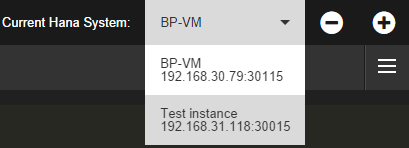
\includegraphics[width=0.6\textwidth]{figures/hana-instances.png}
	\caption{Auswahl-Menü für verschiedene Datenbank-Server}
	\label{fig:hanainstances}
\end{figure}

